%---------------------------------------------------------------------------
% MBS Benchmark A01: Simple Pendulum
%---------------------------------------------------------------------------
%
% LaTeX Template: Jacobs Landscape Poster
% Created by:
% Computational Physics and Biophysics Group, Jacobs University
% https://teamwork.jacobs-university.de:8443/confluence/display/CoPandBiG/LaTeX+Poster


\documentclass[final]{beamer}

\usepackage[scale=1.24]{beamerposter} % Use the beamerposter package for laying out the poster

\usetheme{confposter} % Use the confposter theme supplied with this template

\setbeamercolor{block title}{fg=ngreen,bg=white} % Colors of the block titles
\setbeamercolor{block body}{fg=black,bg=white} % Colors of the body of blocks
\setbeamercolor{block alerted title}{fg=white,bg=dblue!70} % Colors of the highlighted block titles
\setbeamercolor{block alerted body}{fg=black,bg=dblue!10} % Colors of the body of highlighted blocks
% Many more colors are available for use in beamerthemeconfposter.sty
 

\newlength{\sepwid}
\newlength{\onecolwid}
\newlength{\twocolwid}
\newlength{\threecolwid}
\setlength{\paperwidth}{48in} % A0 width: 46.8in
\setlength{\paperheight}{36in} % A0 height: 33.1in
\setlength{\sepwid}{0.024\paperwidth} % Separation width (white space) between columns
\setlength{\onecolwid}{0.301\paperwidth} % Width of one column
\setlength{\twocolwid}{0.602\paperwidth} % Width of two columns
\setlength{\threecolwid}{0.903\paperwidth} % Width of three columns
\setlength{\topmargin}{-0.5in} % Reduce the top margin size
%-----------------------------------------------------------

\usepackage{graphicx}  % Required for including images
\graphicspath{{../MBSfigures/}}
\usepackage{booktabs} % Top and bottom rules for tables

\usepackage{multirow}
\usepackage{siunitx}

\title{MBS Benchmark A01: Simple Pendulum} % Poster title


%----------------------------------------------------------------------------------------

\begin{document}

%\addtobeamertemplate{block end}{}{\vspace*{2ex}} % White space under blocks
%\addtobeamertemplate{block alerted end}{}{\vspace*{2ex}} % White space under highlighted (alert) blocks

\setlength{\belowcaptionskip}{2ex} % White space under figures
\setlength\belowdisplayshortskip{2ex} % White space under equations

\begin{frame}[t] % The whole poster is enclosed in one beamer frame

\begin{columns}[t] % The whole poster consists of three major columns, the second of which is split into two columns twice - the [t] option aligns each column's content to the top

\begin{column}{\sepwid}\end{column} % Empty spacer column

\begin{column}{\twocolwid} % The first column

%----------------------------------------------------------------------------------------
%	OBJECTIVES
%----------------------------------------------------------------------------------------

\begin{alertblock}{Benchmark Objective}
The NMS benchmark problem \textbf{A01} is a simple planar pendulum, proposed as a demonstration example.
\end{alertblock}



%----------------------------------------------------------------------------------------
%    BENCHMARK DESCRIPTION
%----------------------------------------------------------------------------------------


\begin{columns}[t, totalwidth=\twocolwid]

\begin{column}{0.95\onecolwid}
\begin{block}{Benchmark Description}
The Simple Pendulum (Fig.\ref{FIG:SimplePendulum}) is a planar mechanism composed of a point mass linked to the ground through a rigid massless bar. Tab.~\ref{TAB:SystemProperties} reports system configuration. Gravity is the only force applied to the mechanism.


\end{block}


\begin{figure}
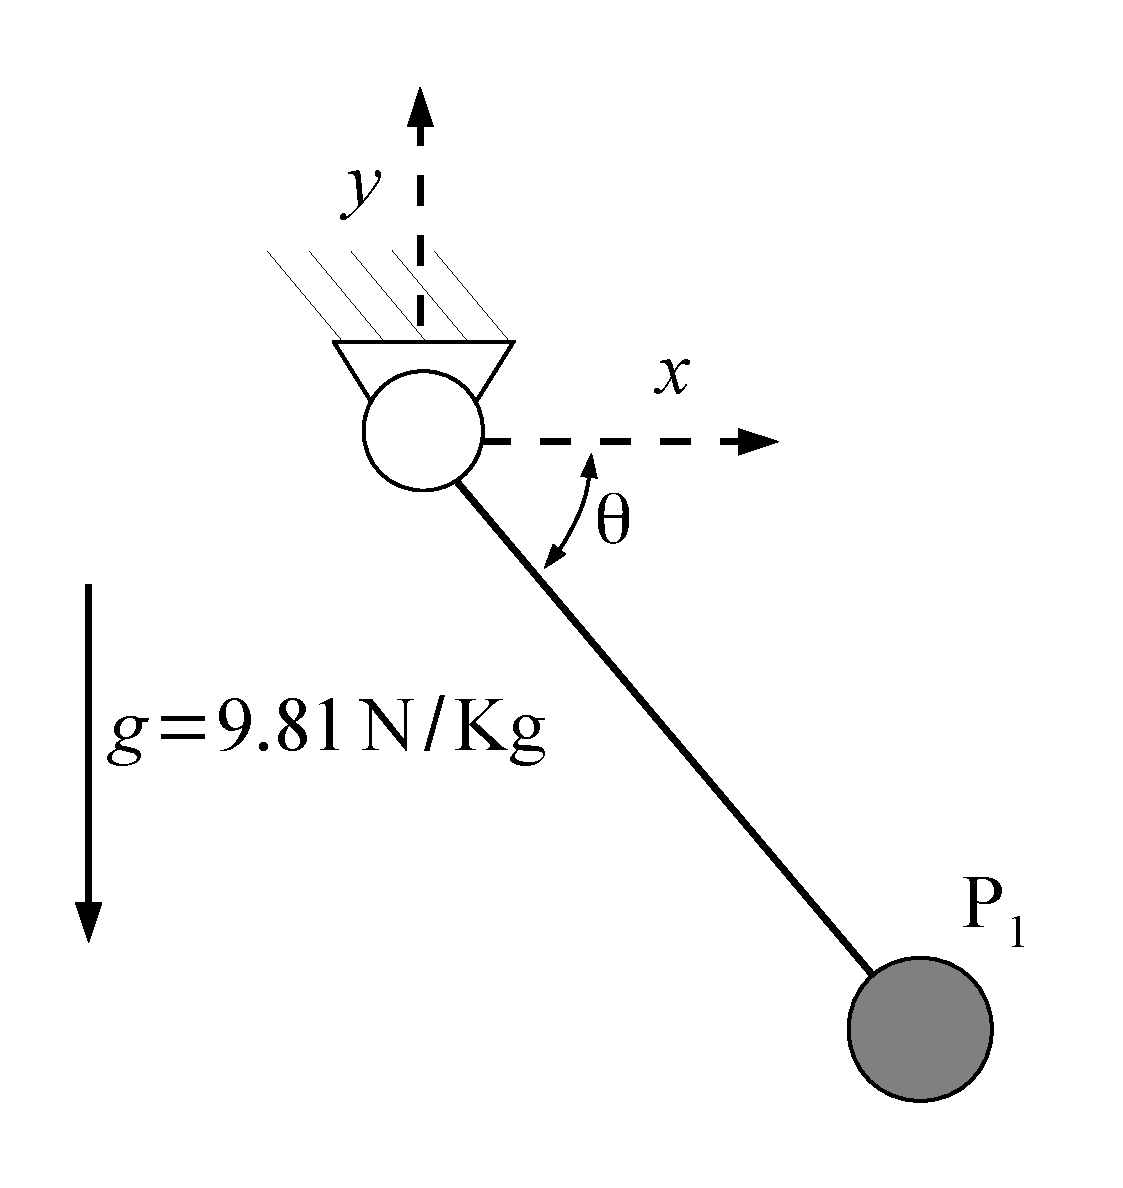
\includegraphics[width=0.8\linewidth]{1MBS_Pendolum}
\caption{Simple Pendulum sketch.}
\label{FIG:SimplePendulum}
\end{figure}

\begin{table}
\begin{large}
\vspace{2ex}
\qquad\qquad
\begin{tabular}[b]{ll}
% \multicolumn{2}{c}{\textbf{System Configuration}}\\
\toprule
$P_1$ mass & $\SI{1.0}{\kilogram}$\\
Bar lenght & $\SI{1.0}{\meter}$\\
Bar mass & $\SI{0.0}{\kilogram}$\\
$\theta(0)$ & $\SI{0.0}{\radian}$\\
$\dot{\theta}(0)$ & $\SI{0.0}{\radian / \second}$\\
\bottomrule
\end{tabular}
\end{large}
\label{TAB:SystemProperties}
\caption{System Properties and Configuration}
\end{table}


\end{column}

\begin{column}{0.95\onecolwid} %Second Column


%----------------------------------------------------------------------------------------
%    RESULTS
%----------------------------------------------------------------------------------------


\begin{block}{Results}
The dynamic simulation of the \textbf{A01} benchmark was executed for \SI{2000}{\second}.
In the initial position, the system is horizontal with $P_1$~\mbox{x-coordinate} equals to \SI{1.0}{\meter}.
Fig.~\ref{FIG:simulationPlot} shows the outputs of OpenSim-based simulation and the benchmark references~\cite{gonzalez2006benchmarking} for a \SI{10}{\second} period.


\begin{figure}[h]
\centering
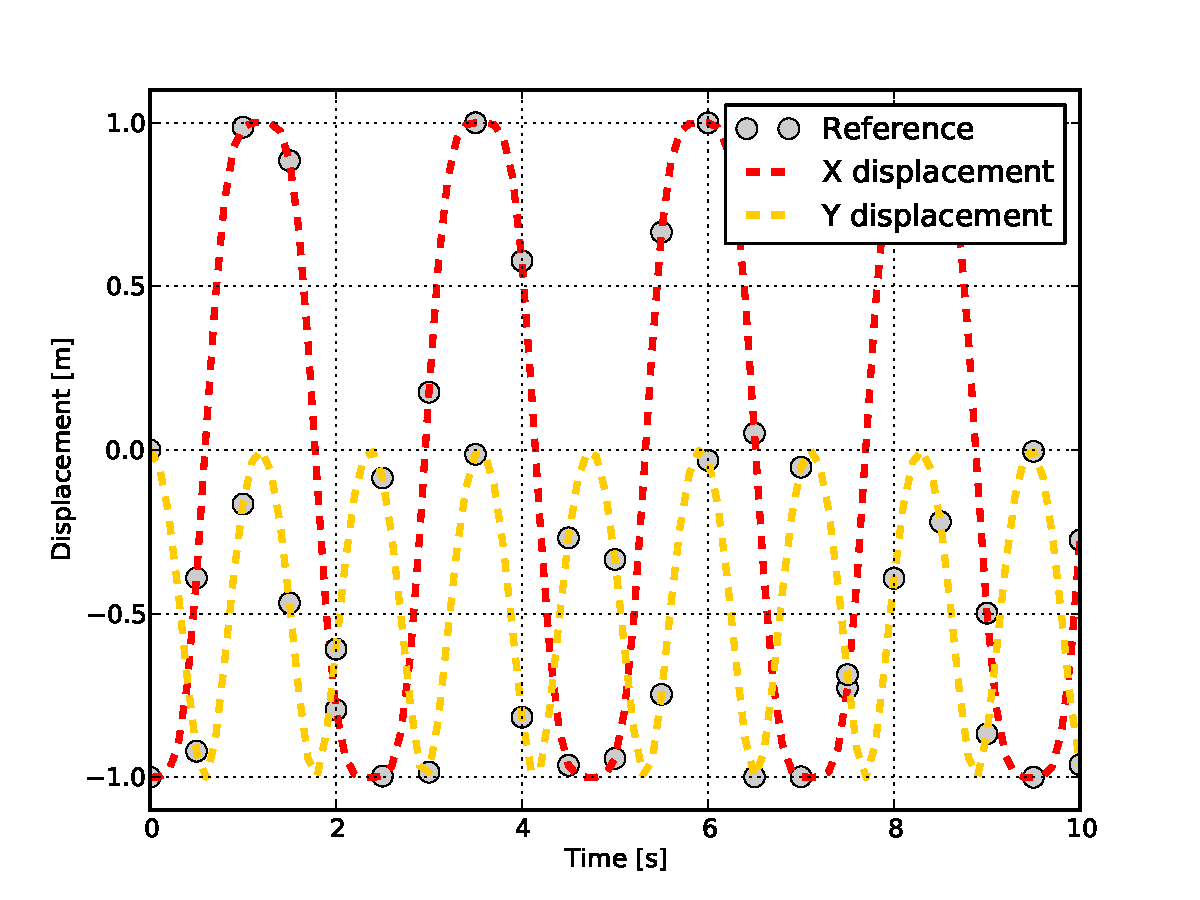
\includegraphics[width=0.95\textwidth]{1MBS_resultsPlot.pdf}
\caption{$P_1$ coordinate displacements in OpenSim simulation (dashed lines) and MBS benchmark reference (gray dots)}. 
\label{FIG:simulationPlot}
\end{figure}

\end{block}

\end{column}
\end{columns}
\end{column}


\begin{column}{0.95\onecolwid} % The third column
\begin{block}{Download}
\begin{itemize}
\item MBS Benchmark available at: \url{http://goo.gl/ySQ5me}
\item OpenSim implementation available at: \url{http://goo.gl/R9tl3z}
\item Videos of OpenSim simulation available at: \url{http://goo.gl/DIIWA7}
\end{itemize}
\end{block}

\begin{block}{References}

\begin{thebibliography}{99}

\bibitem{gonzalez2006benchmarking} M. Gonz{\'a}lez, D. Dopico, U. Lugr{\'\i}s, J. Cuadrado, \textit{``A benchmarking system for MBS simulation software: Problem standardization and performance measurement''} 	in Multibody System Dyn., vol.6, no.2,  2006, pp.~179--190.

\end{thebibliography}

\end{block}

\setbeamercolor{block alerted title}{fg=black,bg=norange} % Change the alert block title colors
\setbeamercolor{block alerted body}{fg=black,bg=white} % Change the alert block body colors

\vspace{36cm}
\begin{alertblock}{Contact Information}
Rehabilitation Engineering Group\\Department of Management and Engineering\\ University of Padua


\begin{itemize}
\item Web: \href{http://reg.gest.unipd.it}{http://reg.gest.unipd.it}
\item Email: \href{mailto:reg.info@gest.unipd.it}{reg.info@gest.unipd.it}
\end{itemize}

\end{alertblock}

%----------------------------------------------------------------------------------------

\end{column} % End of the third column

\end{columns} % End of all the columns in the poster

\end{frame} % End of the enclosing frame

\end{document}
